\let\negmedspace\undefined
\let\negthickspace\undefined
\documentclass[journal]{IEEEtran}
\usepackage[a5paper, margin=10mm, onecolumn]{geometry}
\usepackage{lmodern} % Ensure lmodern is loaded for pdflatex
\usepackage{tfrupee} % Include tfrupee package

\setlength{\headheight}{1cm} % Set the height of the header box
\setlength{\headsep}{0mm}     % Set the distance between the header box and the top of the text

\usepackage{gvv-book}
\usepackage{gvv}
\usepackage{cite}
\usepackage{amsmath,amssymb,amsfonts,amsthm}
\usepackage{algorithmic}
\usepackage{graphicx}
\usepackage{textcomp}
\usepackage{xcolor}
\usepackage{txfonts}
\usepackage{listings}
\usepackage{enumitem}
\usepackage{mathtools}
\usepackage{gensymb}
\usepackage{comment}
\usepackage[breaklinks=true]{hyperref}
\usepackage{tkz-euclide} 
\usepackage{listings}
\usepackage{gvv}                                        
\def\inputGnumericTable{}                       
\usepackage[latin1]{inputenc}                                
\usepackage{color}                                            
\usepackage{array}                                            
\usepackage{longtable}                                       
\usepackage{calc}                                             
\usepackage{multirow}                                         
\usepackage{hhline}                                           
\usepackage{ifthen}                                           
\usepackage{lscape}  
\usetikzlibrary{patterns}
\begin{document}
\bibliographystyle{IEEEtran}


\textbf{Question 2.10.15:} \\
The number of vectors of unit length perpendicular to vectors 
\begin{align}
\vec{a} = (1,1,0) \quad \text{and} \quad \vec{b} = (0,1,1)
\end{align}
is
\begin{align}
\text{(a) one \quad (b) two \quad (c) three \quad (d) infinite \quad (e) None of these}
\end{align}

\textbf{Solution:}\\
 \textbf{Given}  
\begin{solution}
Let
\begin{align}
\vec{a}=\myvec{1\\1\\0},\quad 
\vec{b}=\myvec{0\\1\\1}, \quad
\vec{x}=\myvec{x_1\\x_2\\x_3}.
\end{align}
A vector $\vec{x}$ perpendicular to both $\vec{a}$ and $\vec{b}$ satisfies
\begin{align}
\vec{a}^\top\vec{x} &= 0 
\label{eq:q1-ax0}\\
\vec{b}^\top\vec{x} &= 0 
\label{eq:q1-bx0}
\end{align}
\begin{align}
    \begin{myvec}{\vec{a} &&\vec{b}}^T\end{myvec}\vec{x}=\begin{myvec}{0\\0}
    \end{myvec}
\end{align}
From row reduction

\begin{align}
\vec{x}=\lambda\myvec{-1\\1\\-1}.
\label{eq:q1-dir}
\end{align}
Thus a direction vector is
\begin{align}
\vec{n}=\myvec{-1\\1\\-1},\qquad 
\|\vec{n}\|=\sqrt{3}.
\label{eq:q1-norm}
\end{align}
Hence the \emph{unit} vectors perpendicular to both $\vec{a}$ and $\vec{b}$ are
\begin{align}
\vec{u}=\pm\frac{1}{\sqrt{3}}\myvec{-1\\1\\-1}.
\label{eq:q1-unit}
\end{align}
Therefore, the number of such unit vectors is $\boxed{2}$.
\end{solution}
 
\newpage
\begin{figure}
    \centering
    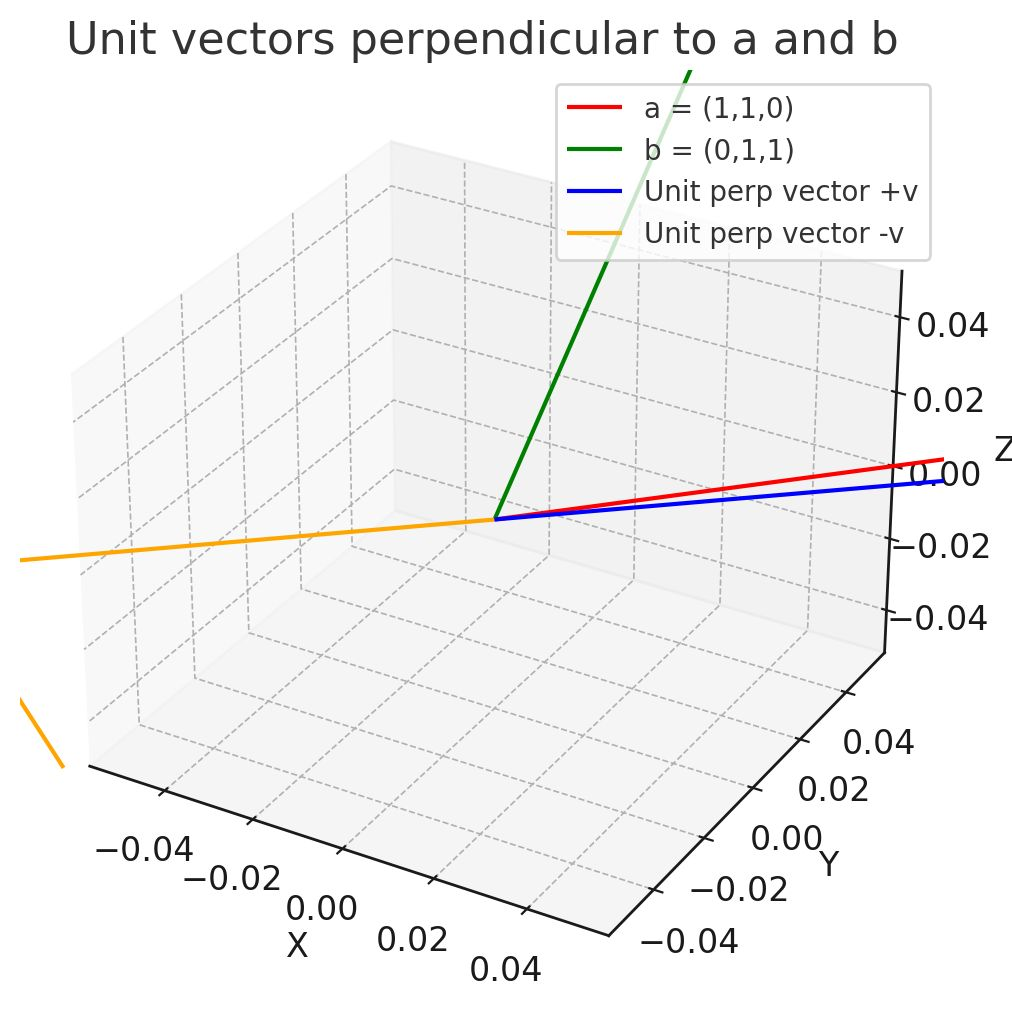
\includegraphics[width=0.5\linewidth]{figs/matg5.jpeg}
    \caption{Caption}
    \label{fig:placeholder}
\end{figure}
\end{document}
